\documentclass[conference]{IEEEtran}
\IEEEoverridecommandlockouts
\usepackage{cite}
\usepackage{amsmath,amssymb,amsfonts}
\usepackage{booktabs}
\usepackage{enumitem}
\usepackage{tikz}
\usetikzlibrary{arrows.meta,positioning}

\newcommand{\sat}{\operatorname{sat}}
\newcommand{\diag}{\operatorname{diag}}
\newcommand{\skewm}[1]{[#1]_\times}

\begin{document}

\title{Quanser QDrone Quadrotor:\\ Hardware Physics, Identification, Modelling, and the Complete Controller Suite\\
{\footnotesize Mathematical foundations for offline simulation, digital-twin, and hardware execution}}

\author{\IEEEauthorblockN{Gandhi Contreras}
\IEEEauthorblockA{\textit{Electrical and Computer Engineering}, New Mexico State University, Las Cruces, NM, USA \\ gandhico@nmsu.edu}}

\maketitle

\begin{abstract}
This paper develops the complete mathematics of the QDrone quadrotor in free flight: the six-degree-of-freedom rigid-body dynamics in the quaternion parameterization, the battery--ESC--brushless-rotor actuation chain with its thrust/torque aerodynamics and mixer allocation, the onboard sensing physics (IMU, optical flow / downward camera, altitude ranging, and external localization) with the estimation structure they impose, identification experiments linear in the parameters, and the full controller suite in the cascaded architecture native to multirotors --- position/velocity outer loops generating attitude and collective-thrust references for the inner attitude loop --- with PID, LQR, LQG, backstepping, sliding-mode, and NMPC formulations, hover linearization, and the free-flight safety envelope.
\end{abstract}

\begin{IEEEkeywords}
QDrone, quadrotor, six-DOF dynamics, differential flatness, cascaded control, LQR, LQG, backstepping, SMC, NMPC.
\end{IEEEkeywords}

%====================================================================
\section{Introduction}
The QDrone is a research quadrotor flown indoors under external or onboard localization. Its mathematics extend the static-mount attitude testbed (companion paper) by the translational degrees of freedom and their coupling: attitude \emph{is} the actuator of translation, since the only force available is the collective thrust along the body axis. States:
\begin{equation}
x = (p,\ v,\ q,\ \omega)\in\mathbb R^3\times\mathbb R^3\times\mathbb S^3\times\mathbb R^3,
\end{equation}
position/velocity in the inertial frame, unit quaternion, body rates. Inputs are the four rotor commands $u\in[0,u_{\max}]^4$.

%====================================================================
\section{Hardware Physics}

\begin{figure*}[!t]
\centering
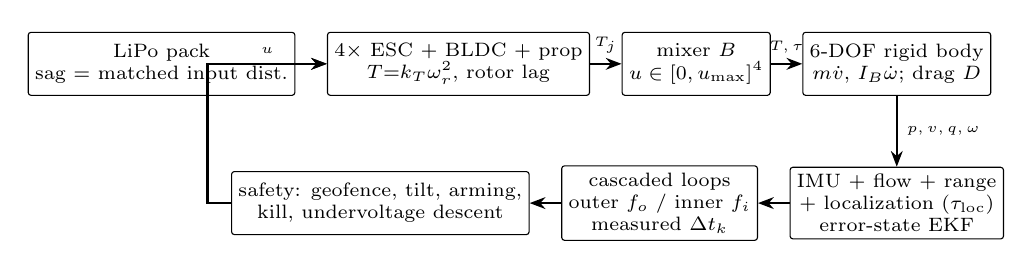
\begin{tikzpicture}[
  node distance=3mm and 4mm,
  blk/.style={draw, rounded corners=1pt, align=center, font=\scriptsize, inner sep=2.5pt, minimum height=8mm},
  lbl/.style={font=\tiny, align=center},
  arr/.style={-{Stealth[length=2mm]}, thick}
]

\node[blk] (bat) {LiPo pack\\ sag = matched input dist.};
\node[blk, right=of bat] (esc) {$4\times$ ESC + BLDC + prop\\ $T{=}k_T\omega_r^2$, rotor lag};
\node[blk, right=of esc] (mix) {mixer $B$\\ $u\in[0,u_{\max}]^4$};
\node[blk, right=of mix] (body) {6-DOF rigid body\\ $m\dot v$, $I_B\dot\omega$; drag $D$};
\node[blk, below=9mm of body] (sens) {IMU + flow + range\\ + localization ($\tau_{\mathrm{loc}}$)\\ error-state EKF};
\node[blk, left=of sens] (loops) {cascaded loops\\ outer $f_o$ / inner $f_i$\\ measured $\Delta t_k$};
\node[blk, left=of loops] (safe) {safety: geofence, tilt, arming,\\ kill, undervoltage descent};
\draw[arr] (bat) -- (esc);
\draw[arr] (esc) -- node[lbl, above] {$T_j$} (mix);
\draw[arr] (mix) -- node[lbl, above] {$T,\tau$} (body);
\draw[arr] (body) -- node[lbl, right] {$p,v,q,\omega$} (sens);
\draw[arr] (sens) -- (loops);
\draw[arr] (loops) -- (safe);
\draw[arr] (safe.west) -- ++(-3mm,0) |- node[lbl, pos=0.75, above] {$u$} (esc.west);
\end{tikzpicture}
\caption{QDrone free-flight signal chain: the estimation stack imposed by the sensing suite feeds the cascaded architecture; allocation clipping and the safety state machine close the loop.}
\label{fig:chain}
\end{figure*}
The actuation chain is that of the static-mount paper, summarized: LiPo pack with sag $V_b = n_s(v_{\mathrm{oc}}(\mathrm{SoC}) - R_{\mathrm{int}}i_b)$; ESC-driven brushless motors, DC-equivalent electrical model and rotor-speed lag $J_r\dot\omega_r = k_t i - k_Q\omega_r^2 - b_r\omega_r$; propeller maps $T_j = k_T\omega_{r,j}^2$, $Q_j = k_Q\omega_{r,j}^2$; mixer
\begin{equation}
[\,T,\ \tau_x,\ \tau_y,\ \tau_z\,]^{\!\top} = B\,u,
\label{eq:mixer}
\end{equation}
inverted with the non-negativity clip $u_j\in[0,u_{\max}]$; rotor gyroscopic and inertial reaction torques as refinements. Manual-verified (QDrone~2): 4S LiPo $3700$~mAh, $45$C rating, undervoltage shutdown below $14$~V (uneven-cell-charge caution below $13.3$~V); motor speed constant $1300$~RPM/V. Free flight adds three physics items with control consequences: (i) \emph{thrust-to-weight}: the collective must both support $mg$ and steer, so attitude authority collapses near the thrust limits --- the allocation constraint is active physics, not bookkeeping; (ii) \emph{aerodynamic drag and blade flapping}: lumped as $F_d = -D\,R^{\!\top}v$ (rotor-frame linear drag), the term that damps translational dynamics and enables drag-aided velocity estimation from the accelerometer; (iii) \emph{battery sag under climb} scales all four thrusts simultaneously --- a matched input disturbance handled by integral action or voltage scheduling.

\subsection{Sensing}
MEMS IMU (gyro/accel with bias random walks) at high rate; downward camera/optical flow giving body-frame velocity at moderate rate; time-of-flight or barometric altitude; and, indoors, external localization (motion capture / UWB) giving $p$ (and heading) at camera rate with latency $\tau_{\mathrm{loc}}$. The estimation structure imposed by this suite is the standard error-state EKF: IMU propagates
\begin{equation}
\dot{\hat p} = \hat v,\quad
\dot{\hat v} = R(\hat q)\,(a_m - b_a) + g e_3,\quad
\dot{\hat q} = \tfrac12\hat q\otimes[0;\,\omega_m - b_g],
\end{equation}
with corrections from flow/range/localization; latency is compensated by state augmentation or measurement re-timing. Safety envelope: geofence on $\hat p$, altitude ceiling/floor, tilt limit, arming interlocks, RC/kill override, undervoltage staged descent, loss-of-localization hover-then-land logic, and prop guards for indoor work.

%====================================================================
\section{Six-DOF Model}
Newton--Euler in mixed coordinates (inertial translation, body rotation):
\begin{align}
m\dot v &= -\,m g\,e_3 + T\,R(q)\,e_3 - R(q) D R(q)^{\!\top} v, \label{eq:trans}\\
\dot q &= \tfrac12\, q\otimes [0;\ \omega], \label{eq:quatkin}\\
I_B\dot\omega &= -\,\omega\times I_B\omega + \tau + \tau_{\mathrm{gyro}}. \label{eq:rot}
\end{align}
with $(T,\tau)$ from \eqref{eq:mixer}. Structure: \eqref{eq:rot} is fully actuated (3 torques, 3 DOF); \eqref{eq:trans} is underactuated --- the force direction is slaved to attitude. The system is \emph{differentially flat} with flat outputs $(p, \psi)$: given any sufficiently smooth position/yaw trajectory, the full state and inputs are algebraic functions of the flat outputs and their derivatives,
\begin{equation}
T = m\,\|\ddot p + g e_3 + \ldots\|,\qquad
z_b^d = \frac{\ddot p + g e_3}{\|\ddot p + g e_3\|},
\label{eq:flat}
\end{equation}
which is the mathematical foundation of trajectory generation and of the cascaded control architecture below.

\subsection{Hover linearization}
About hover ($q = q_0$, $T_0 = mg$, small Euler angles $\phi,\theta$ and yaw $\psi$):
\begin{align}
\ddot x^{(i)} &= g\,\theta,\qquad \ddot y^{(i)} = -g\,\phi,\qquad \ddot z^{(i)} = \Delta T/m,\nonumber\\
I_{xx}\ddot\phi &= \tau_x,\qquad I_{yy}\ddot\theta = \tau_y,\qquad I_{zz}\ddot\psi = \tau_z,
\label{eq:hoverlin}
\end{align}
four decoupled chains: two fourth-order lateral channels (torque $\to$ angle $\to$ acceleration), one second-order heave, one second-order yaw --- the design plant for the linear suite, assembled as $\dot x = Ax + Bu'$ with $u' = [\Delta T,\ \tau^{\!\top}]^{\!\top}$.

%====================================================================
\section{Identification}

\begin{figure}[!t]
\centering
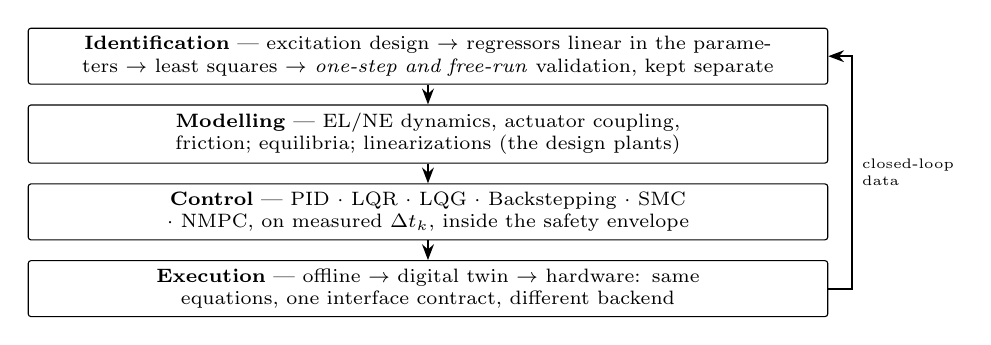
\begin{tikzpicture}[
  node distance=2.5mm,
  blk/.style={draw, rounded corners=1pt, align=center, font=\scriptsize, inner sep=3pt, text width=0.82\columnwidth},
  arr/.style={-{Stealth[length=2mm]}, thick}
]
\node[blk] (id) {\textbf{Identification} --- excitation design $\to$ regressors linear in the parameters $\to$ least squares $\to$ \emph{one-step and free-run} validation, kept separate};
\node[blk, below=of id] (mod) {\textbf{Modelling} --- EL/NE dynamics, actuator coupling, friction; equilibria; linearizations (the design plants)};
\node[blk, below=of mod] (ctl) {\textbf{Control} --- PID $\cdot$ LQR $\cdot$ LQG $\cdot$ Backstepping $\cdot$ SMC $\cdot$ NMPC, on measured $\Delta t_k$, inside the safety envelope};
\node[blk, below=of ctl] (exe) {\textbf{Execution} --- offline $\to$ digital twin $\to$ hardware: same equations, one interface contract, different backend};
\draw[arr] (id) -- (mod);
\draw[arr] (mod) -- (ctl);
\draw[arr] (ctl) -- (exe);
\draw[arr] (exe.east) -- ++(3mm,0) |- node[font=\tiny, pos=0.25, right, align=left] {closed-loop\\ data} (id.east);
\end{tikzpicture}
\caption{The workflow every platform in this series follows: identification feeds modelling, modelling feeds the controller suite, and all stages run unchanged across the three execution targets; closed-loop records return to identification.}
\label{fig:workflow}
\end{figure}
E1) \emph{rotor maps} $k_T, k_Q$ and lag on a thrust stand across $V_b$; E2) \emph{mass/inertia}: scale and bifilar-pendulum swings; on-vehicle refinement by regressing \eqref{eq:rot} over torque doublets (linear in $I_{xx},I_{yy},I_{zz}$); E3) \emph{drag} $D$: level constant-speed flights, regress \eqref{eq:trans} against EKF velocity (linear in $D$); E4) \emph{hover trim}: rotor offsets and c.o.m. bias from steady hover commands; E5) black-box per-axis ARX cross-checks on \eqref{eq:hoverlin}; validation always as one-step and free-run separately on held-out flights.

%====================================================================
\section{Control Suite: Cascaded Architecture}
Native structure (justified by \eqref{eq:flat} and time-scale separation): an outer position/velocity loop at rate $f_o$ produces the desired specific force $f_d = \ddot p_d + g e_3$, mapped to $(T_c, q_r)$ by \eqref{eq:flat} with the commanded yaw; the inner attitude loop (companion static-mount paper, same equations) tracks $q_r$ at rate $f_i \gg f_o$; the mixer allocates. All discrete updates on measured $\Delta t_k$.

\subsection{PID}
Outer loop per axis:
$f_d = \ddot p_r + K_d(\dot p_r - \hat v) + K_p(p_r - \hat p) + K_i\!\int(p_r-\hat p)\,dt$,
integral with anti-windup against the tilt and thrust limits (the saturations couple: the achievable $f_d$ set is a cone). Inner loop: quaternion PD $\tau = -K_q e_q - K_\omega\omega$ with bandwidth-based gains as validated on our campaigns.

\subsection{LQR / LQG}
On \eqref{eq:hoverlin}: per-channel LQR (lateral channels are 4-state chains $[p, v, \angle, \dot\angle]$), weights by Bryson scaling of position/tilt/torque bounds; the full 12-state coupled design is the same CARE with block structure. LQG: the error-state EKF of the sensing section \emph{is} the estimator; separation nominally, with the localization latency margin verified against the loop delay budget.

\subsection{Backstepping}
The cascade made rigorous: $z_1 = p - p_r$, virtual $v_d = \dot p_r - c_1 z_1$; $z_2 = \hat v - v_d$ defines $f_d = \ddot p_r - c_2 z_2 - z_1$; the attitude subsystem backsteps $z_3 = e_q(q, q_r(f_d))$, $z_4 = \omega - \omega_d$ exactly as in the static-mount paper, with the interconnection term bounded by the tilt limit. Composite $V = \tfrac12\sum\|z_i\|^2_{(\cdot)}$ gives $\dot V \le -\sum c_i\|z_i\|^2 + $ cross terms dominated for $c_{3,4}$ sufficiently large --- the formal content of ``inner loop faster than outer.''

\subsection{Sliding mode}
Per lateral channel, composite surface $s = (\tfrac{d}{dt} + \lambda)^{3}(p - p_r)$ (relative degree 4) or, practically, cascade SMC: outer $s_o = \dot e_p + \lambda_o e_p$ shaping $f_d$, inner $s_i = \omega_e + \Lambda_i e_q$ shaping $\tau$; boundary layers set above IMU/flow noise floors; reaching gains sized to the identified rotor-map and drag uncertainties.

\subsection{NMPC}
Receding horizon on \eqref{eq:trans}--\eqref{eq:rot} (or on \eqref{eq:hoverlin} for linear MPC), RK4 at $\Delta t_p$:
\begin{align}
\min_{\{u_k\}}\ \sum_{k=0}^{N-1}&\Bigl(\|p_k - p_{r,k}\|_{Q_p}^2 + \|v_k\|_{Q_v}^2 + \|e_{q,k}\|_{Q_q}^2 \nonumber\\
&+ \|\omega_k\|_{Q_\omega}^2 + \|u_k - u_h\|_R^2\Bigr) + V_f(x_N)
\end{align}
s.t. $u\in[0,u_{\max}]^4$, tilt cone, geofence as state constraints. NMPC subsumes the cascade: allocation, tilt, and thrust constraints are handled in one problem, which is precisely where it outperforms the cascade near actuator limits (aggressive waypoints, recovery). Real-time reductions as validated on our other platforms: short horizon, move blocking, warm start from the shifted solution, terminal cost from the hover LQR.

%====================================================================
\section{Execution Modes and Conclusion}
Offline: \eqref{eq:trans}--\eqref{eq:rot} with rotor lags, battery sag, sensor noise/latency models injectable. Digital twin: the vendor virtual QDrone under the same command/measurement contract. Hardware: staged commissioning --- bench (props off), tethered/guarded hover, free flight --- under the safety envelope; sign conventions and mixer orientation are verified prop-off first. The equations above constitute the complete mathematical basis: six-DOF dynamics with flatness, hover linearization, parameter-linear identification, and the six-controller suite in the cascaded architecture.

\bibliographystyle{IEEEtran}
\begin{thebibliography}{9}
\bibitem{mahony2012} R.~Mahony, V.~Kumar, and P.~Corke, ``Multirotor aerial vehicles,'' \emph{IEEE Robot. Autom. Mag.}, 2012.
\bibitem{mellinger2011} D.~Mellinger and V.~Kumar, ``Minimum snap trajectory generation and control for quadrotors,'' \emph{IEEE ICRA}, 2011.
\bibitem{markley2014} F.~L. Markley and J.~L. Crassidis, \emph{Fundamentals of Spacecraft Attitude Determination and Control}. Springer, 2014.
\bibitem{quanser_qdrone} Quanser Consulting Inc., \emph{QDrone 2 User Manual}, Markham, ON, Canada.
\bibitem{khalil2002} H.~K. Khalil, \emph{Nonlinear Systems}, 3rd ed. Prentice Hall, 2002.
\bibitem{krstic1995} M.~Krsti\'c, I.~Kanellakopoulos, and P.~Kokotovi\'c, \emph{Nonlinear and Adaptive Control Design}. Wiley, 1995.
\bibitem{utkin1992} V.~Utkin, \emph{Sliding Modes in Control and Optimization}. Springer, 1992.
\bibitem{rawlings2017} J.~B. Rawlings, D.~Q. Mayne, and M.~Diehl, \emph{Model Predictive Control}, 2nd ed. Nob Hill, 2017.
\end{thebibliography}

\end{document}
